%!TEX root = ../main.tex

\section{Modeling of Factor Returns} % (fold)
\label{sec:modeling_of_factor_returns}

% Why a model?
This section presents our model for the joint behavior of returns. A multivariate model of returns allows us to make conditional forecasts of the distribution of returns one week ahead, which take into account the dependence between factors. The model is used in the mean-variance analysis, to provide dynamic inputs that can give us optimal weights over time. The model is also used in the analysis of diversification benefits, when we shift the focus to the tail risk of factor portfolios. First, we describe why we choose the copula model among different multivariate models. Second, we describe the building blocks of the model and analyze which specification best suits the dependence structure in the data. Last, we provide estimates and describe the model we retain for further use.

\subsection{Choosing a multivariate model}
% Why copula?
The ARMA-GARCH family of models has become the norm of modeling univariate financial return series, beginning with \textcite{Bollerslev1986}. The straightforward extension of univariate GARCH models to multiple return series has, however, proven difficult. Unrestricted multivariate GARCH (MGARCH) models that model the conditional covariance matrix directly become impossible to estimate as the number of covariances grows exponentially with the number of series. It thus becomes necessary to restrict the parameter space, where the BEKK model is a common example~\autocite{BEKKModel}.

% Separate modeling of variance and correlation
A parsimonious solution to the dimensionality problem is to separate the modeling of return and volatility dynamics from the modeling of conditional correlations. The separation allows for consistent (albeit inefficient) two-step estimation, and makes large-scale estimation feasible. One such approach is the \emph{dynamic conditional correlation} (DCC) model originally proposed by~\autocite{Engle2002}. In the DCC model, univariate GARCH models are first estimated on each series. Then, an autoregressive process for the correlation matrix is fitted to the standardized residuals ${z_t}$ of those models. 

% Asymmetric cDCC and copula cDCC
DCC is a useful and tractable model for estimating time-varying correlations between return series. However, it is a model of correlations only and is not flexible enough to model the univariate components differently. More specifically, it is not constructed to generate tail dependence, which is the notion that correlation dynamics can be very different in extreme realizations. 

% Enter the copula
Copula models have recently attracted much attention in the field of risk management, as they provide a flexible way to infer a multivariate probability distribution. Copula models are, just like DCC models, based on two-step estimation and work well in large scale applications. Furthermore, copulae are flexible enough to generate tail dependence, which is shown to be an important feature of factor return data~\autocite{ChristoffersenLanglois2013}. 

Copula models are most often constructed by estimating univariate models from the ARMA-GARCH family in the first step. The residuals from the ARMA-GARCH models are then used in the copula function that explains the multivariate dependence, including dynamic correlations and tail dependence.

We choose to work with a copula model, as it can (1) estimate the joint distribution function in large scale applications, (2) model different univariate models for the different factors, and (3) incorporate both tail dependence and dynamic correlations. Next, we define and describe the copula model.

\subsection{Definition of the copula model}
This is section 05_04, but adapted so that ARMA-GARCH is explained when needed.
\subsection{Univariate models}
This describes the selection and estimation of the univariate models.
\subsection{Analysis and choice of dependence structure}
This is the work on residuals from the univariate models, and is what makes us believe that a certain dependence structure is right.
\subsection{Copula estimation results}
Here the main tables that show which model to prefer, discuss parameter estimates.
\subsection{Robustness check of copula}
Here simulated threshold correlations?
\subsection{Model retained for further use}
Here describe again the model we use in MV and CDB. E.g. dynamic std. If the reader doesn't follow anything of the first four subsections, she should at least be able to pick up what we use here.
%
%!TEX root = ../main.tex

\subsection{Copula Modeling of Dependency} % (fold)
\label{sub:05_04_copula}

\subsubsection{Copula Model Specification}

We now turn to modeling the dependency between factors using a copula model. 
Each week, the joint behavior of returns $R_{t+1}$ in the next week is modeled by a joint density function $f_t(R_{t+1})$. Assuming returns are multivariate normally distributed, this would correspond to the multivariate normal density function, fully parametrised by means, volatility and correlation matrix. But neither factor returns $R_t$, nor the standardized returns $z_t$ are normally distributed.

Copulas are a convenient way of modeling dependency between non-normal returns. Following~\textcite{ChristoffersenErrunzaJacobLanglois2012}, who builds on~\textcite{Patton2006} and~\textcite{Sklar1959}, we decompose the joint density function into the product of a joint copula function $c_t$ of uniform variables $U_{t+1}$ and the marginal univariate distributions $f_{i,t}(r_{i, t+1})$:
\begin{align}
  f_t(R_{t+1}) &=
    c_t(U_{t+1}) \prod^N_{i = 1} f_{i,t}(r_{i, t + 1})
\end{align}
The marginal densities, $f_{i,t}(r_{i, t + 1})$, are modeled by ARMA-GARCH processes while the copula $c_t$ is a model of the joint behavior of their probability integral transforms. $c_t$ can be modeled, and estimated, separately from the marginal densities. This is key to imposing a more sophisticated dependency structure on the returns.

After ARMA-GARCH filtering, the marginal densities of returns are modeled by the constant density functions of standardized returns. The vector of uniforms are therefore related to returns by the probability integral transform (PIT) of standardized returns:
\begin{align}
  u_{i, t+1} = \int_{-\infty}^{z_{i,t+1}} f_{i}(z_{i,t+1})
\end{align}
In the most general case, we use a multivariate skewed Student's t \emph{dynamic asymmetric copula} model introduced by~\textcite{ChristoffersenErrunzaJacobLanglois2012}. The joint distribution is parametrised by a single degrees of freedom parameter $\nu_c$, an $N$ vector of skewness parameters $\gamma_{c}$ and a (time-varying) correlation matrix $\Psi_{t}$. We describe the details of the copula distribution in~\autoref{app:ghstmv}.

The normal and Student's t copula are nested in this model, as when $\gamma_{c,i} = 0$, we obtain a multivariate Student's t distribution, and if additionally $\nu_c = \infty$, we obtain the multivariate standard normal distribution.

The copula is made dynamic by evolving the correlation matrix $\Psi_t$ according to an underlying \emph{c}DCC process $Q_t$~\autocites[cf.]{Engle2002,Aielli2013}. Using the notation from~\textcite{ChristoffersenLanglois2013}:\footnote{The difference between ${z_t^*}$ and ${\bar{z}_t^*}$ is due to the \emph{corrected} DCC model; details in the appendix.}
\begin{align}
  Q_t &= (1 - \alpha - \beta) Q
    + \beta Q_{t - 1}
    + \alpha \bar{z}_{t - 1}^* \bar{z}_{t - 1}^{*\top}
  \label{eq:copula_cdcc}
\end{align}
where $Q_t$ is normalized to the correlation matrix
\begin{align}
  \Psi_t = Q_t^{-1/2} Q_t Q_t^{-1/2}
  \label{eq:copula_cdcc_psi}
\end{align}
The $Q_t$ process is comprised of three components that are weighted according to $\alpha, \beta$: (1) a time-invariant component $Q$, (2) an innovation component from copula shocks $\bar{z}_{t-1}^{*} \bar{z}_{t-1}^{*\top}$ and (3) an autoregressive component of order one $Q_{t-1}$. In order for the the correlation matrix $\Psi_t$ to be positive definite, $Q_t$ has to be positive definite, which is ascertained by requiring that $\alpha \geq 0$, $\beta \geq 0$ and $(\alpha + \beta) < 1$. The model nests a constant copula by forcing $\alpha = \beta = 0$.

% XXX NOTATION
% XXX cDCC correction for copula shocks
The parameters of the copula model -- the distribution parameters of the multivariate skewed Student's t distribution and the dynamics parameters of the \emph{c}DCC -- are estimated by maximizing the log-likelihood:
\begin{align}
  \arg\!\max_{\nu_c, \gamma_{ic}, \alpha, \beta} \sum_{t = 1}^T \ln c_t(U_t; \nu_c, \gamma_{ic}, \alpha, \beta)
\end{align}
This estimation takes the uniform residuals from each GARCH model as given. The process of copula estimation with \emph{c}DCC dynamics is quite involved. A detailed description can be found~\autoref{app:copula_cdcc}.

Clearly, the interpretation of the copula parameters is closely associated to the structure of multivariate dependence. By different restrictions on the parameters in the DAC model, we are able to activate or deactivate certain features of the copula: First, the degree of freedom parameter $nu_c$ is to be interpreted as a the measure of tail dependency. When $nu \neq 0$, the lower and upper tails of the joint distribution are fatter than in the normal case, which is coherent with the evidence from threshold correlations in. Second, the skewness parameters $\gamma_{c,i}$ are to be interpreted as the extent of asymmetry in the correlation structure. When $\gamma \neq 0$, there is asymmetry in correlations, which is also coherent with the earlier threshold correlation analysis. Third, the $\alpha$ and $\beta$ parameters determine whether the copula generates time-varying correlations. If $\alpha \neq 0$ and $\beta \neq 0$, the copula is dynamic, which is consistent with the findings of the rolling correlation analysis

\subsubsection{Copula Estimation Results}

We estimate constant and dynamic normal, symmetric and asymmetric copula models on the full dataset of GARCH uniform residuals; results are in~\autoref{tab:copula_estimation}. Looking at the parameter estimates, few of the $\gamma_c$ estimates appear significant, however, $\nu_c$ is clearly not infinite. Additionally, there is little improvement in log-likelihood by going from a symmetric to asymmetric copula. We conclude that the symmetric Student's t copula model is preferred. The insignificance of $\gamma$ can be interpreted as evidence of low asymmetries in the dependency -- or, more likely, that the model is simply unable to capture it.

There is a significant improvement in log-likelihood by going from a constant to dynamic copula, which suggests that time-varying tail dependency is an important feature to capture. The persistence, $\alpha + \beta$ is close to one, which could suggest that the dependency structure of factors is not stationary. We now turn to investigating how well the copula reproduces the dependency patterns observed in the data.

%!TEX root = ../../main.tex

\begin{table}[!ht]
  \centering
  \scriptsize
  \renewcommand{\arraystretch}{1.2}

  \caption{Parameter estimates for copula models based on uniform residuals from ARMA-GJR-GARCH models.\\ \quad \\
  Stationary bootstrap standard errors in parentheses, following Politis and Romano (1994). Copula parameters: $\nu_c$ is the degree of freedom, $\gamma_c$ is the vector of skewness parameters, $\alpha$, $\beta$ are the shock loading and autoregressive loading of the cDCC process. The significance test of $\nu_c$ is based on $1/\nu_c$, as this ratio goes to zero when $\nu_c$ goes to infinity (normality). Sample: 1963-07-05--2016-07-01.}
  \begin{tabularx}{\textwidth}{@{}l ddd X ddd @{}}
    \toprule
    &
      \multicolumn{3}{c}{Constant Copula} &&
      \multicolumn{3}{c}{Dymamic Copula} \\
    \cmidrule{2-4} \cmidrule{6-8}
    &
      \multicolumn{1}{c}{Normal} & \multicolumn{1}{c}{Symmetric \emph{t}} & \multicolumn{1}{c}{Skewed \emph{t}} & &
      \multicolumn{1}{c}{Normal} & \multicolumn{1}{c}{Symmetric \emph{t}} & \multicolumn{1}{c}{Skewed \emph{t}} \\
    \midrule
    $\nu_c$ & & 6.625^{**} & 6.671^{**} && & 11.936^{**} & 11.881^{**} \\
    & & (0.636) & (0.264) && & (0.770) & (0.641) \\
    \\
    $\gamma_\text{Mkt}$ & & & -0.057 && & & -0.078 \\
    & & & (0.047) && & & (0.062) \\
    \\
    $\gamma_\text{HML}$ & & & 0.103 && & & 0.083 \\
    & & & (0.036) && & & (0.071) \\
    \\
    $\gamma_\text{SMB}$ & & & -0.103 && & & -0.175 \\
    & & & (0.055) && & & (0.098) \\
    \\
    $\gamma_\text{Mom}$ & & & -0.202^{**} && & & -0.145 \\
    & & & (0.032) && & & (0.073) \\
    \\
    $\gamma_\text{RMW}$ & & & 0.021 && & & 0.095 \\
    & & & (0.035) && & & (0.058) \\
    \\
    $\gamma_\text{CMA}$ & & & 0.076 && & & 0.001 \\
    & & & (0.038) && & & (0.050) \\
    \\
    $\alpha$ & & & && 0.065 & 0.068^{**} & 0.068^{**} \\
    & & & && (0.006) & (0.006) & (0.006) \\
    \\
    $\beta$ & & & && 0.915 & 0.913^{**} & 0.913^{**} \\
    & & & && (0.008) & (0.007) & (0.007) \\
    \midrule
    Log-likelihood & 1169.194 & 1555.683 & 1572.672 && 2790.618 & 2977.648 & 2989.273 \\
    No. of Parameters & 15 & 16 & 22 && 17 & 18 & 24 \\
    % BIC & -348.32 & -122.21 & -316.432 && -243.221 & -342.342 & -396.324 \\
    Persistence & & & && 0.981 & 0.981 & 0.981 \\
    \bottomrule
  \end{tabularx}

  \label{tab:copula_estimation}
\end{table}



% subsection copula_model (end)

%!TEX root = ../main.tex

\subsection{Univariate Modeling of Returns} % (fold)
\label{sub:univariate_modeling_of_returns}

We proceed by estimating models of each factor's return series and attempt to capture the effects of non-normality, autocorrelation and volatility clustering that were established in \autoref{sec:data}. From a modeling perspective, these effects suggest that the conditional density of each factor's return series $f_{i,t}(r_{i,t+1})$ are not time-varying. By estimating ARMA-GARCH, we can characterize and filter these effects. Furthermore, we can incorporate the effects in conditional forecasts. After filtering, we are left with the \emph{standardized returns} of each factor, $z_{i,t}$, which are assumed to be independent over time, i.e. described by constant density functions $f_i(z_{i,t})$.

\subsubsection{General univariate model: ARMA-GJR-GARCH}

The ARMA-GARCH is a broad model family designed to eliminate predictable components of financial return series, originally introduced by~\textcite{Bollerslev1986}. The models use autoregressive and moving average lags to capture serial correlation in return data (ARMA), as well as autoregressive and moving average lags to capture ARCH effects in residuals from the mean equation (GARCH). Shocks in financial return series are often not homoskedastic, and the heteroskedasticy tends to exhibit serial correlation. We evaluate the GJR-GARCH model of~\textcite{glosten1993relation}, which is a parsimonious extension of the standard GARCH(1, 1). The GJR-GARCH is designed to also capture leverage effects~\autocite{glosten1993relation}, i.e. when positive and negative return shocks have different impact on future volatility~\autocite{Black1976}.

We estimate conditional mean equations for each factor \emph{up to} ARMA(3, 3):
\begin{align}
  r_{i,t} &=
    \phi_{i,0} +
    \sum^p \phi_{i,p} r_{i,t - p} +
    \sum^q \theta_{i,q} \varepsilon_{i,t - q} + 
    \varepsilon_{i,t}
    \label{eq:garch_mean}
\end{align}
where $r_{i,t}$ are weekly returns of each factor. The conditional volatility evolves according to the GJR-GARCH specification:
\begin{align}
  \varepsilon_{i,t} &= \sigma_{i,t} z_{i,t} \\
  \sigma_{i,t}^2 &=
    \omega_i +
    (\alpha_i + \eta_i I_{\varepsilon_{i,t-1} \leq 0}) \varepsilon_{i,t - 1}^2 +
    \beta_{i} \sigma^2_{i,t - 1}
    \label{eq:garch_garch}
\end{align}
where $I$ is an indicator function that is equal to one when $\varepsilon_{i,t-1} \leq 0$. A positive $\eta_i$ captures the leverage effect by increasing the current period's volatility if the previous period's residual $\varepsilon_{i,t-1}$ was below zero. A significant $\eta_i$ thus introduces asymmetric volatility in the model. For the market factor, it is expected that $\eta_i$ is positive, reflecting the leverage effect in the market itself and no impact from the short risk-free component. However, for the other factors, which are constructed as all-equity zero-cost long-short portfolios, the direction of $\eta_i$ is less obvious~\autocite{ChristoffersenLanglois2013}. If there are leverage effects for stocks in general, negative shocks will lead to more volatility than positive shocks in a portfolio of stocks. But in a zero-cost portfolio, the leverage effects of the long positions in stocks could be eliminated by the short positions in other firms. The level of the leverage effect in a zero-cost portfolio therefore depends on the relative strength of leverage effects in the long and short components.

% XXX In the estimation, we also use variance targeting as proposed by~\textcite{EngleMezrich1995}, which is shown makes optimization faster and sometimes more certain to reach the global maximum. This means that $\omega$ is not estimated in the maximum likelihood setting, but instead set to 1 minus the persistence of the process times the sample mean of squared residuals, where the persistence is $\alpha + \beta$ for the GARCH.\footnote{Note that in the case of the GJR-GARCH for the Mkt-RF factor, the persistence is $\alpha + \beta + \eta \kappa$ where $\kappa$ is the probability that standardized residuals $z_t$ are below zero.}
The ARMA-GARCH models are estimated on each series using maximum likelihood estimation, with assumed distributions of standardized returns $z_{i,t}$. We evaluate models where the standardized returns are assumed to follow one of the following distributions: Standard normal, Student's \textit{t} with $\nu$ degrees of freedom and skewed Student's \textit{t} with $\nu$ degrees of freedom and skewness $\gamma$. The Student's t distribution allows for greater kurtosis (fatter tails) than the standard normal distribution, while skewed Student's \textit{t} also allows for additional asymmetry in the model's behavior beyond that introduced by the leverage effect~\autocite{ChristoffersenErrunzaJacobLanglois2012}. Details about the skewed Student's t distribution, which we also use in our copula model, can be found in~\autoref{app:ghstmv}

\subsubsection{Factor specific model selection process}

Our selection process is as follows: For each factor strategy, we estimate GJR-GARCH models on the full dataset ($T = 2766$) up to ARMA(3, 3) and GARCH(1, 1) under normal, Student's t and skewed Student's t residuals, with and without $\eta_i$ fixed to zero (in which case we obtain the basic GARCH(1,~1) model). We then compute the Bayesian Information Criterion~\autocite[BIC]{Schwarz1978} for each factor strategy and specification and select the ARMA order with the lowest BIC as our primary candidates.

First, the candidate models are checked for remaining serial correlation and ARCH effects. Second, we examine whether there are significant leverage effects that warrant the use of a GJR-GARCH instead of a standard GARCH. Third, we use QQ-plots to control for misspecification in the residual process, and to find a suitable distribution for the standardized residuals $z_t$.

In a well-specified model, we expect there to be no significant serial correlation, ARCH effects or sign bias in the residuals. We employ weighted Ljung-Box, ARCH LM and sign bias tests that are detailed in \autoref{app:univariate_diagnostics}. Furthermore, the QQ-plots of the standardized residuals should show that their empirical distribution is comparable to the assumed theoretical distribution (be distributed around the 45 degree line).

\subsubsection{Model selection and estimation results}

The result of our selection and estimation procedure are presented in~\autoref{tab:garch_estimation}. The Mkt-RF factor is the only model that requires a GJR-GARCH $\eta_i \neq 0$, while the remaining models are all standard GARCH (1, 1). The minimization of BIC leads to ARMA(0, 0) for Mkt-RF, ARMA(1, 0) for Mom and CMA and ARMA(1, 1) for the remaining factors HML, SMB, RMW. 



\begin{table}[!ht]
  \centering
  \scriptsize
  \renewcommand{\arraystretch}{1.2}

  \caption{Parameter estimates from ARMA-GARCH models in~\autoref{eq:garch_mean}and \autoref{eq:garch_garch} of weekly returns.\\ \quad \\
  Heteroskedasticity robust standard errors in parentheses, following \textcite{White1982}. Sample: 1963-07-05--2016-07-01 (2766 weekly obs). $\gamma$ and $\nu$ are the skewness and degree of freedom parameters of the skewed Student's \textit{t} innovations. $\eta$ is fixed at zero, as the sign bias test showed no significant misspecification of the GARCH for the HML, RMW and CMA factors. $\omega$ is set using variance targeting, following \textcite{EngleMezrich1995}. \emph{UV} is the estimate of unconditional volatility; \emph{VP} is the estimate of variance persistence. Ljung-Box and ARCH-LM tests are the weighted portmanteau tests from \textcite{FisherGallagher2012} and the sign bias test is from \textcite{EngleNg1993}, see appendix for details. Note: $^{*}$p$<$0.1; $^{**}$p$<$0.05; $^{***}$p$<$0.01}
  \begin{tabularx}{\textwidth}{@{}l X dddddd @{}}
    \toprule
    &&
      \multicolumn{1}{c}{Mkt.RF} &
      \multicolumn{1}{c}{SMB} &
      \multicolumn{1}{c}{Mom} &
      \multicolumn{1}{c}{HML} &
      \multicolumn{1}{c}{CMA} &
      \multicolumn{1}{c}{RMW} \\
    \midrule
    $\mu$ (\%) && 0.115^{***} & 0.032 & 0.137^{***} & 0.064^{**} & 0.040^{***} & 0.055^{***} \\
               && (0.031) & (0.032) & (0.046)& (0.025) & (0.012) & (0.016) \\
               \\
    $\phi_1$   &&         & 0.773^{***} & 0.129^{***} & 0.723^{***} & 0.111^{***} & 0.589^{***}\\
               &&         & (0.045) & (0.049) & (0.081) & (0.020) & (0.190) \\
               \\
    $\theta_1$ &&         & -0.651^{***} &      &   -0.610^{***} & & -0.466^{**} \\
               &&         & (0.056) &     &    (0.090)  & & (0.210) \\
               \\
    $\alpha$   && 0.032^{**} & 0.114^{***} & 0.183^{***} & 0.109^{***} & 0.088^{***} & 0.077^{***} \\
               && (0.014) & (0.023) & (0.008) & (0.002) & (0.002) & (0.002) \\
               \\
    $\beta$    && 0.845^{***} & 0.842^{***} & 0.796^{***} & 0.873^{***} & 0.899^{***} & 0.915^{***} \\
               && (0.007) & (0.035) & (0.009) & (0.002) & (0.001) & (0.001) \\
               \\
    $\eta$     && 0.189^{***} &  & \\
               && (0.024) &  & & \\
               \\
    $\gamma$   && -2.356^{**} & -0.650 & -2.124 & 0.627 & 0.484 & 0.248 \\
               && (0.836) & (1.036) & (9.898) & (0.405) & (0.493) & (0.421) \\
               \\
    $\nu$      && 13.246^{***} & 11.564 & 13.356 & 10.197^{***} & 11.094^{***} & 10.949^{*}\\
               && (3.505) & (12.085) & (40.035) & (2.669) & (3.481) & (5.652) \\
               \\
    $\omega\,\,(\text{permil}) $   && 0.016 & 0.006 & 0.007 & 0.003 & 0.001 & 0.001 \\
               && \\
    \midrule
    LLH  && \multicolumn{1}{r}{7,051} & \multicolumn{1}{r}{8,567} & \multicolumn{1}{r}{7,941} & \multicolumn{1}{r}{8,788} & \multicolumn{1}{r}{9,574} & \multicolumn{1}{r}{9,872} \\
    UV   && 0.022 & 0.010 & 0.017 & 0.010 & 0.010 & 0.010 \\
    VP   && 0.968 & 0.957 & 0.979 & 0.982 & 0.987 & 0.992 \\
    \midrule
    \multicolumn{8}{@{}l}{\textbf{p-values of Ljung-Box (LB), ARCH-LM and Sign Bias tests}} \\
    LB(5)          && 0.148 & 0.271 & 0.828 & 1.000 & 0.182 & 1.000 \\
    LB(10)         && 0.098 & 0.720 & 0.721 & 0.977 & 0.070 & 0.055 \\
    ARCH-LM(5)     && 0.812 & 0.626 & 0.053 & 0.117 & 0.837 & 0.724 \\
    ARCH-LM(10)    && 0.931 & 0.882 & 0.134 & 0.391 & 0.945 & 0.911 \\
    Sign bias [-]  && 0.883 & 0.331 & 0.836 & 0.094 & 0.473 & 0.204 \\
    Sign bias [+]  && 0.156 & 0.094 & 0.381 & 0.399 & 0.069 & 0.648 \\
    \bottomrule
  \end{tabularx}

  \label{tab:garch_estimation}
\end{table}


Based on these ARMA-GARCH specifications, the Ljung-Box and LM tests indicate no remaining serial correlation or ARCH effects, as all p-values are greater than our 5\% cut-off point. However, some p-values are quite close to the limit, including the Mkt-RF factor's Ljung-Box tests and the longer Ljung-Box tests of RMW and CMA.

The lack of significant sign bias in the GARCH specifications for all models except Mkt-RF is interesting, but in line with the argument that any leverage effects could cancel out in a zero-cost long-short equity portfolio; the Mkt-RF is the only factor that is net-long equities and also exhibited the expected negative sign bias as a GARCH model. We note that the sign bias of Mkt-RF has been eliminated in the GJR-GARCH model. Notably, all factors exhibit high values of $\alpha_i$ and $\beta_i$ indicating highly persistent variance, suggesting there is an opportunity for ``timing volatility''.


Looking at~\autoref{fig:garch_qq}, the candidate specifications under normal and Student's \textit{t} distributed innovations all display misaligned QQ-plots. The empirical distributions deviate from the 45 degree theoretical lines, especially in the more extreme quantiles. This indicates asymmetry in the residual series. In unreported results, we have controlled that the misspecification of normal and Student's \textit{t} residuals is persistent even if GJR-GARCH models are fitted for all factors -- leverage effects cannot explain the misspecification. By comparison, the QQ-plot with skewed Student's \textit{t} innovations seems to fit the data well. We proceed with skewed Student's \textit{t} residual distributions.

\begin{figure}[!pt]
  \centering

  \begin{subfigure}{0.70\textwidth}
    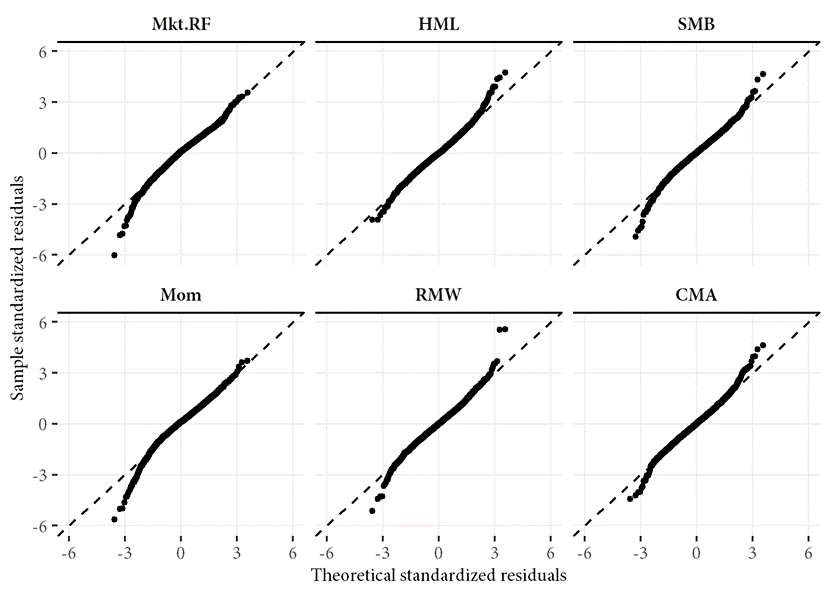
\includegraphics[width=\textwidth]{graphics/qq_norm.png}
    \caption{Normal}
  \end{subfigure}
  \\
  \begin{subfigure}{0.70\textwidth}
    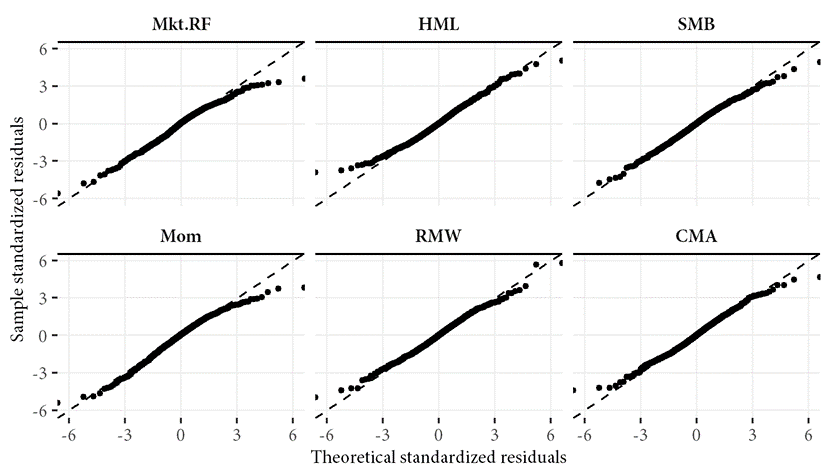
\includegraphics[width=\textwidth]{graphics/qq_std.png}
    \caption{Students't}
  \end{subfigure}
  \\
  \begin{subfigure}{0.70\textwidth}
    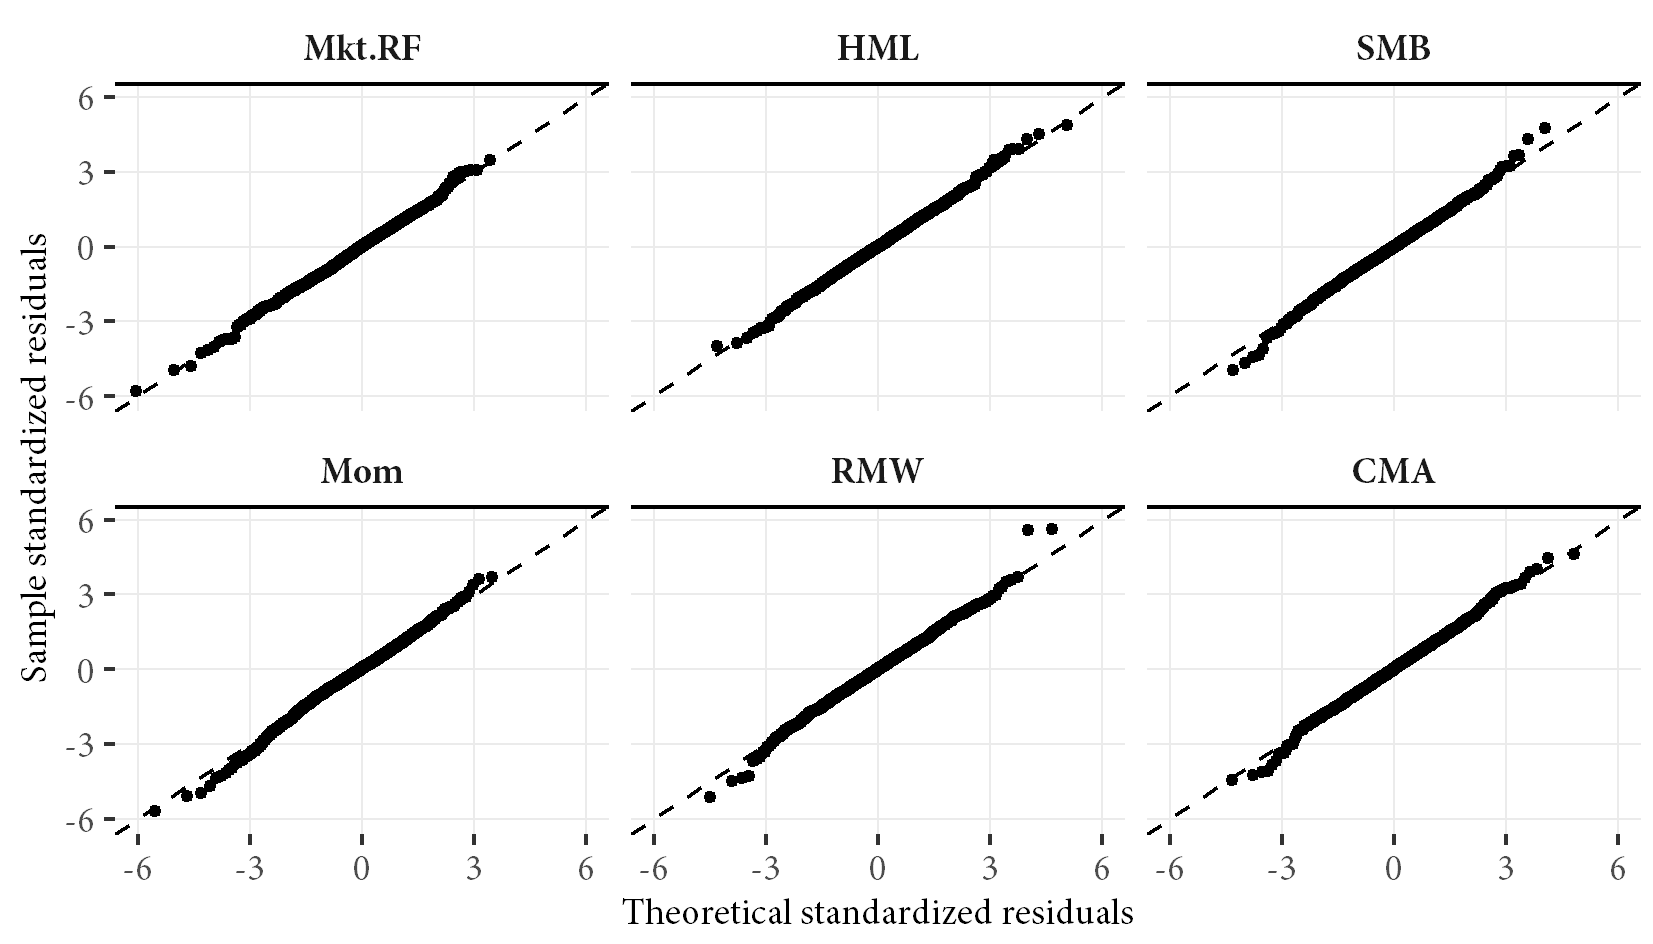
\includegraphics[width=\textwidth]{graphics/qq_ghst.png}
    \caption{Skewed Student's t}
  \end{subfigure}

  \caption{Quantile-quantile plots of theoretical standardized residuals and standardized residuals from the best (lowest BIC) ARMA-GARCH model specifications, with normal, Student's and skewed Student's t innovations. Data from the theoretical distribution should line up on the dashed line. Based on weekly data 1963-2016}
  \label{fig:garch_qq}
\end{figure}

% In the variance equation, all factors exhibit high $\alpha$ and $\beta$ leading to a high variance persistence, between 0.96 and 0.99. Generally, variance persistence, which is related to volatility clustering, tends to be high in financial return series. [WHAT DOES IT MEAN WHY DO I CARE] We note that the zero-cost factor portfolios are no exception. The HML factor has a higher $\alpha$ estimate, indicating that shocks of equal size translate into slightly stronger volatility for HML than for RMW and CMA. RMW, on the other hand, has both the lowest $\alpha$ estimate and the highest $\beta$ estimate, indicating higher persistence and lower sensitivity of volatility to shocks.

% We note that the Mkt-RF factor is, according to our model selection procedure, best fitted by a ARMA(0, 0) mean equation, indicating no predictive power of 1-week lagged returns. Also, in the variance equation, we note that the relatively low $\alpha = 0.037$ sensitivity to shocks is increased considerably by $\eta = 0.181$ in the case of a \emph{negative} shock. Furthermore, the Mom factor stands out with a much higher estimate of $\alpha$ (0.186) than any of the other series (all around 0.10) and a lower $\beta$ (0.793). This means that volatility in the momentum factor is more sensitive than other factor strategies to return shocks and less predictable by past volatility alone. We also note that the Mkt-RF and Mom factors exhibit relatively higher unconditional volatilities (of 0.022 and 0.018) than do other factors (around 0.010).

For both the value-related and non-value related factors, many of the estimates of $\gamma_i$, the skewness of the skewed Student's \textit{t} GARCH innovation process, are statistically insignificant. This is also the case for the degree of freedom estimates for SMB and Mom. Although these parameters are not significantly estimated, we believe that including them is essential as QQ-plots indicate misspecification for models with both the normal and Student's \textit{t} innovations.

% subsection univariate_modeling_of_returns (end)

%!TEX root = ../main.tex

\subsection{Threshold and Rolling Correlations of Residuals} % (fold)

In this subsection, we demonstrate that the standardized residuals ${z_t}$ from ARMA-GARCH models display both tail dependence, measured by threshold correlations, and time-varying correlations, measured by rolling correlations; features we will attempt to model in the copula model. In the context of modeling, we are interested in the standardized returns, rather than the returns themselves, as they are filtered of the variance dynamics present in the returns themselves~\autocite{ChristoffersenLanglois2013}.\footnote{The visual patterns for both threshold and rolling correlations are quite similar between returns and standardized returns; results are available in the appendix.}

\subsubsection{Threshold Correlations}

Threshold (or exceedance) correlations have previously been used to highlight the asymmetric dependence structure of i.a. country equity indices~\autocite{LonginSolnik2001}, portfolios by industry, size, value and momentum~\autocite{AngChen2002} and factor strategies~\autocite{ChristoffersenLanglois2013}. The following analysis is still new as it adds the factors investment (CMA) and profitability (RMW). We follow~\textcite{ChristoffersenLanglois2013} definition of threshold correlation
\begin{align}
    ThCorr(r_i, r_j) = 
    \begin{cases} 
        Corr\Big(r_i, r_j \,|\, r_i < F_i^{-1}(p), r_j < F_j^{-1}(p)\Big)  & \text{for } p < 0.5 \\
        Corr\Big(r_i, r_j \,|\, r_i \geq F_i^{-1}(p), r_j \geq F_j^{-1}(p)\Big)  & \text{for } p \geq 0.5
    \end{cases}
\end{align}
where $F_i^{-1}(p)$ the empirical quantile of $r_i$ at percentile $p$. Threshold correlations thus reflect how series correlate when both are realizing in their respective tails. This subsetting of data is illustrated in \autoref{fig:illustrate_threshold}. In the left hand plots, we see the scatter of ARMA-GARCH residuals of Mkt-RF and HML respectively, and how $p$, found on the $x$-axis of the right hand plot, determines the subset of data that is included in the correlation calculation. We note that the standard correlation, given by the dashed line in the right hand plot, is clearly negative, while threshold correlations in the first and third quadrants are significantly more positive, which shows that not taking threshold correlations into account provides a vaguer picture of the dependence structure when both factor series realize in their tails.

\begin{figure}[!ht]
  \centering
  \footnotesize
  \caption{Illustration of threshold correlations on ARMA-GARCH residuals from the Mkt-RF--HML asset pair, with 95\% confidence bounds. The unconditional correlation is given by the dashed line. Based on weekly data 1963--2016.}
  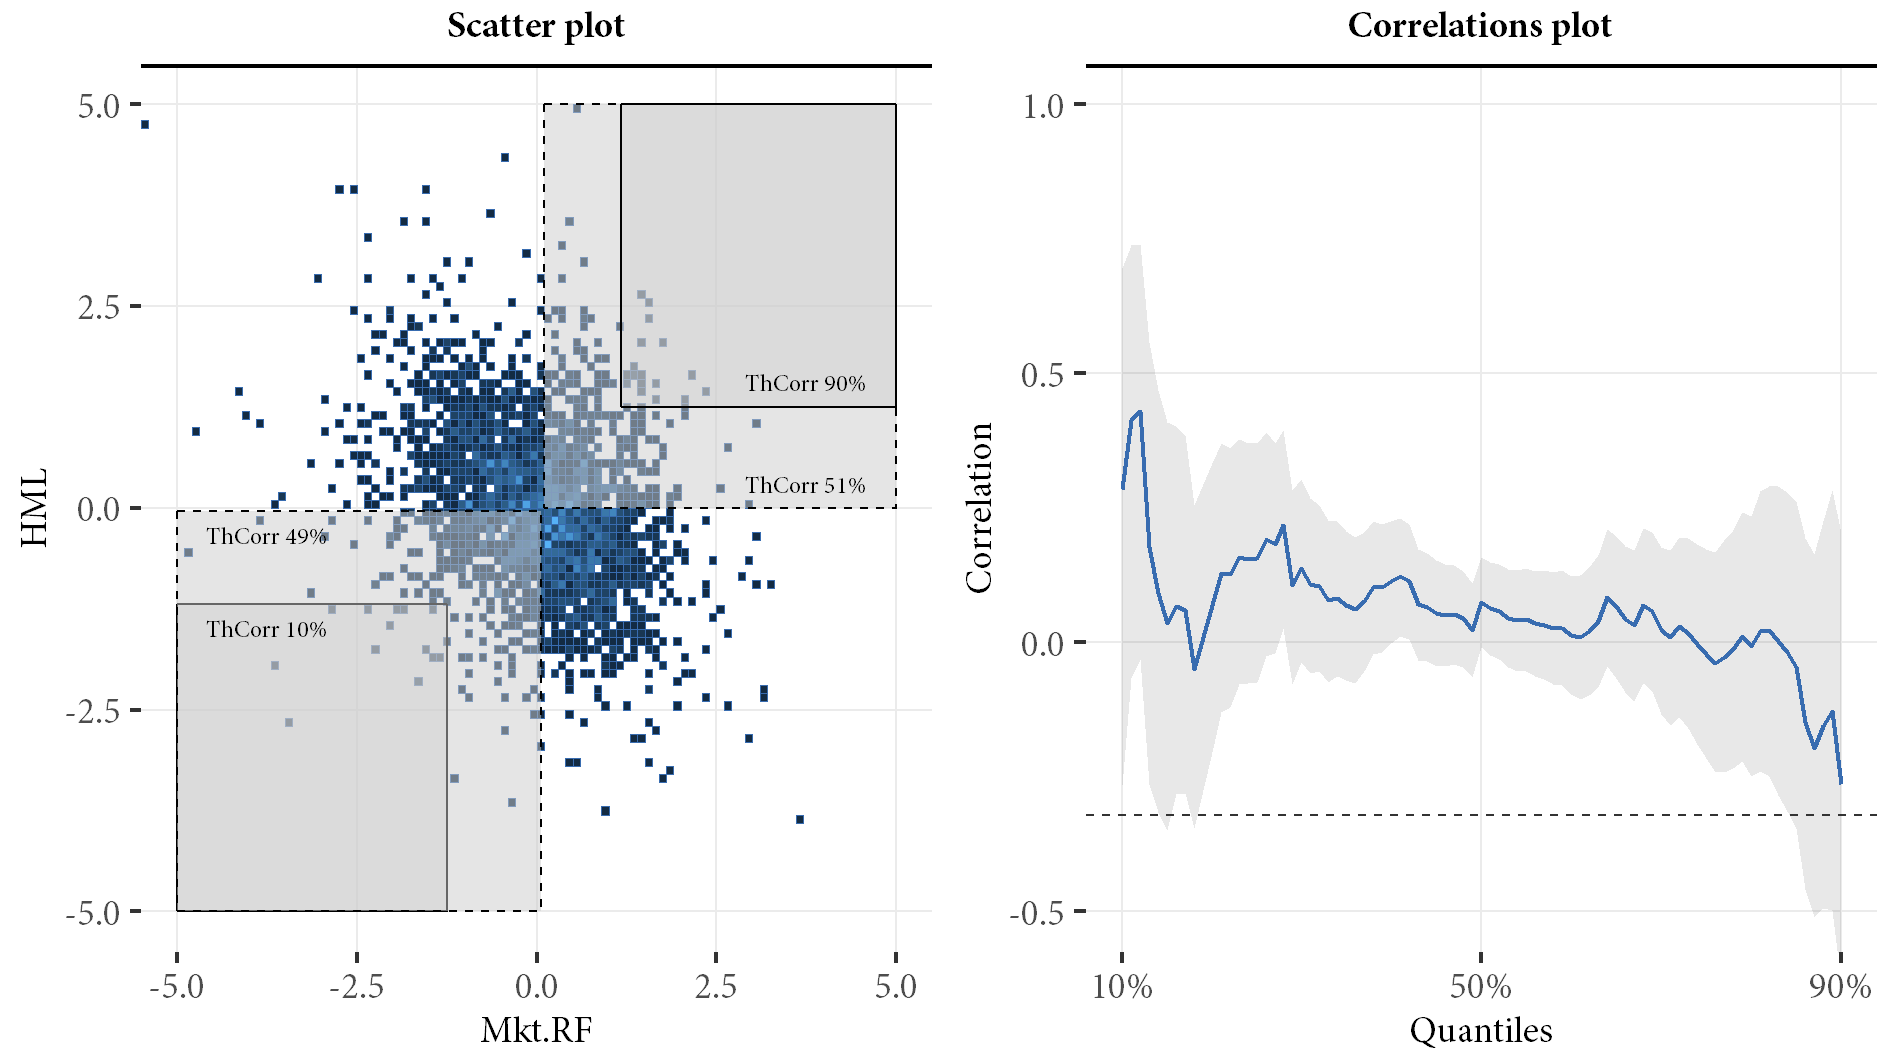
\includegraphics[scale=1]{graphics/threshold_explain_res.png}
  \label{fig:illustrate_threshold}
\end{figure}

\begin{figure}[!ht]
  \centering
  \footnotesize
  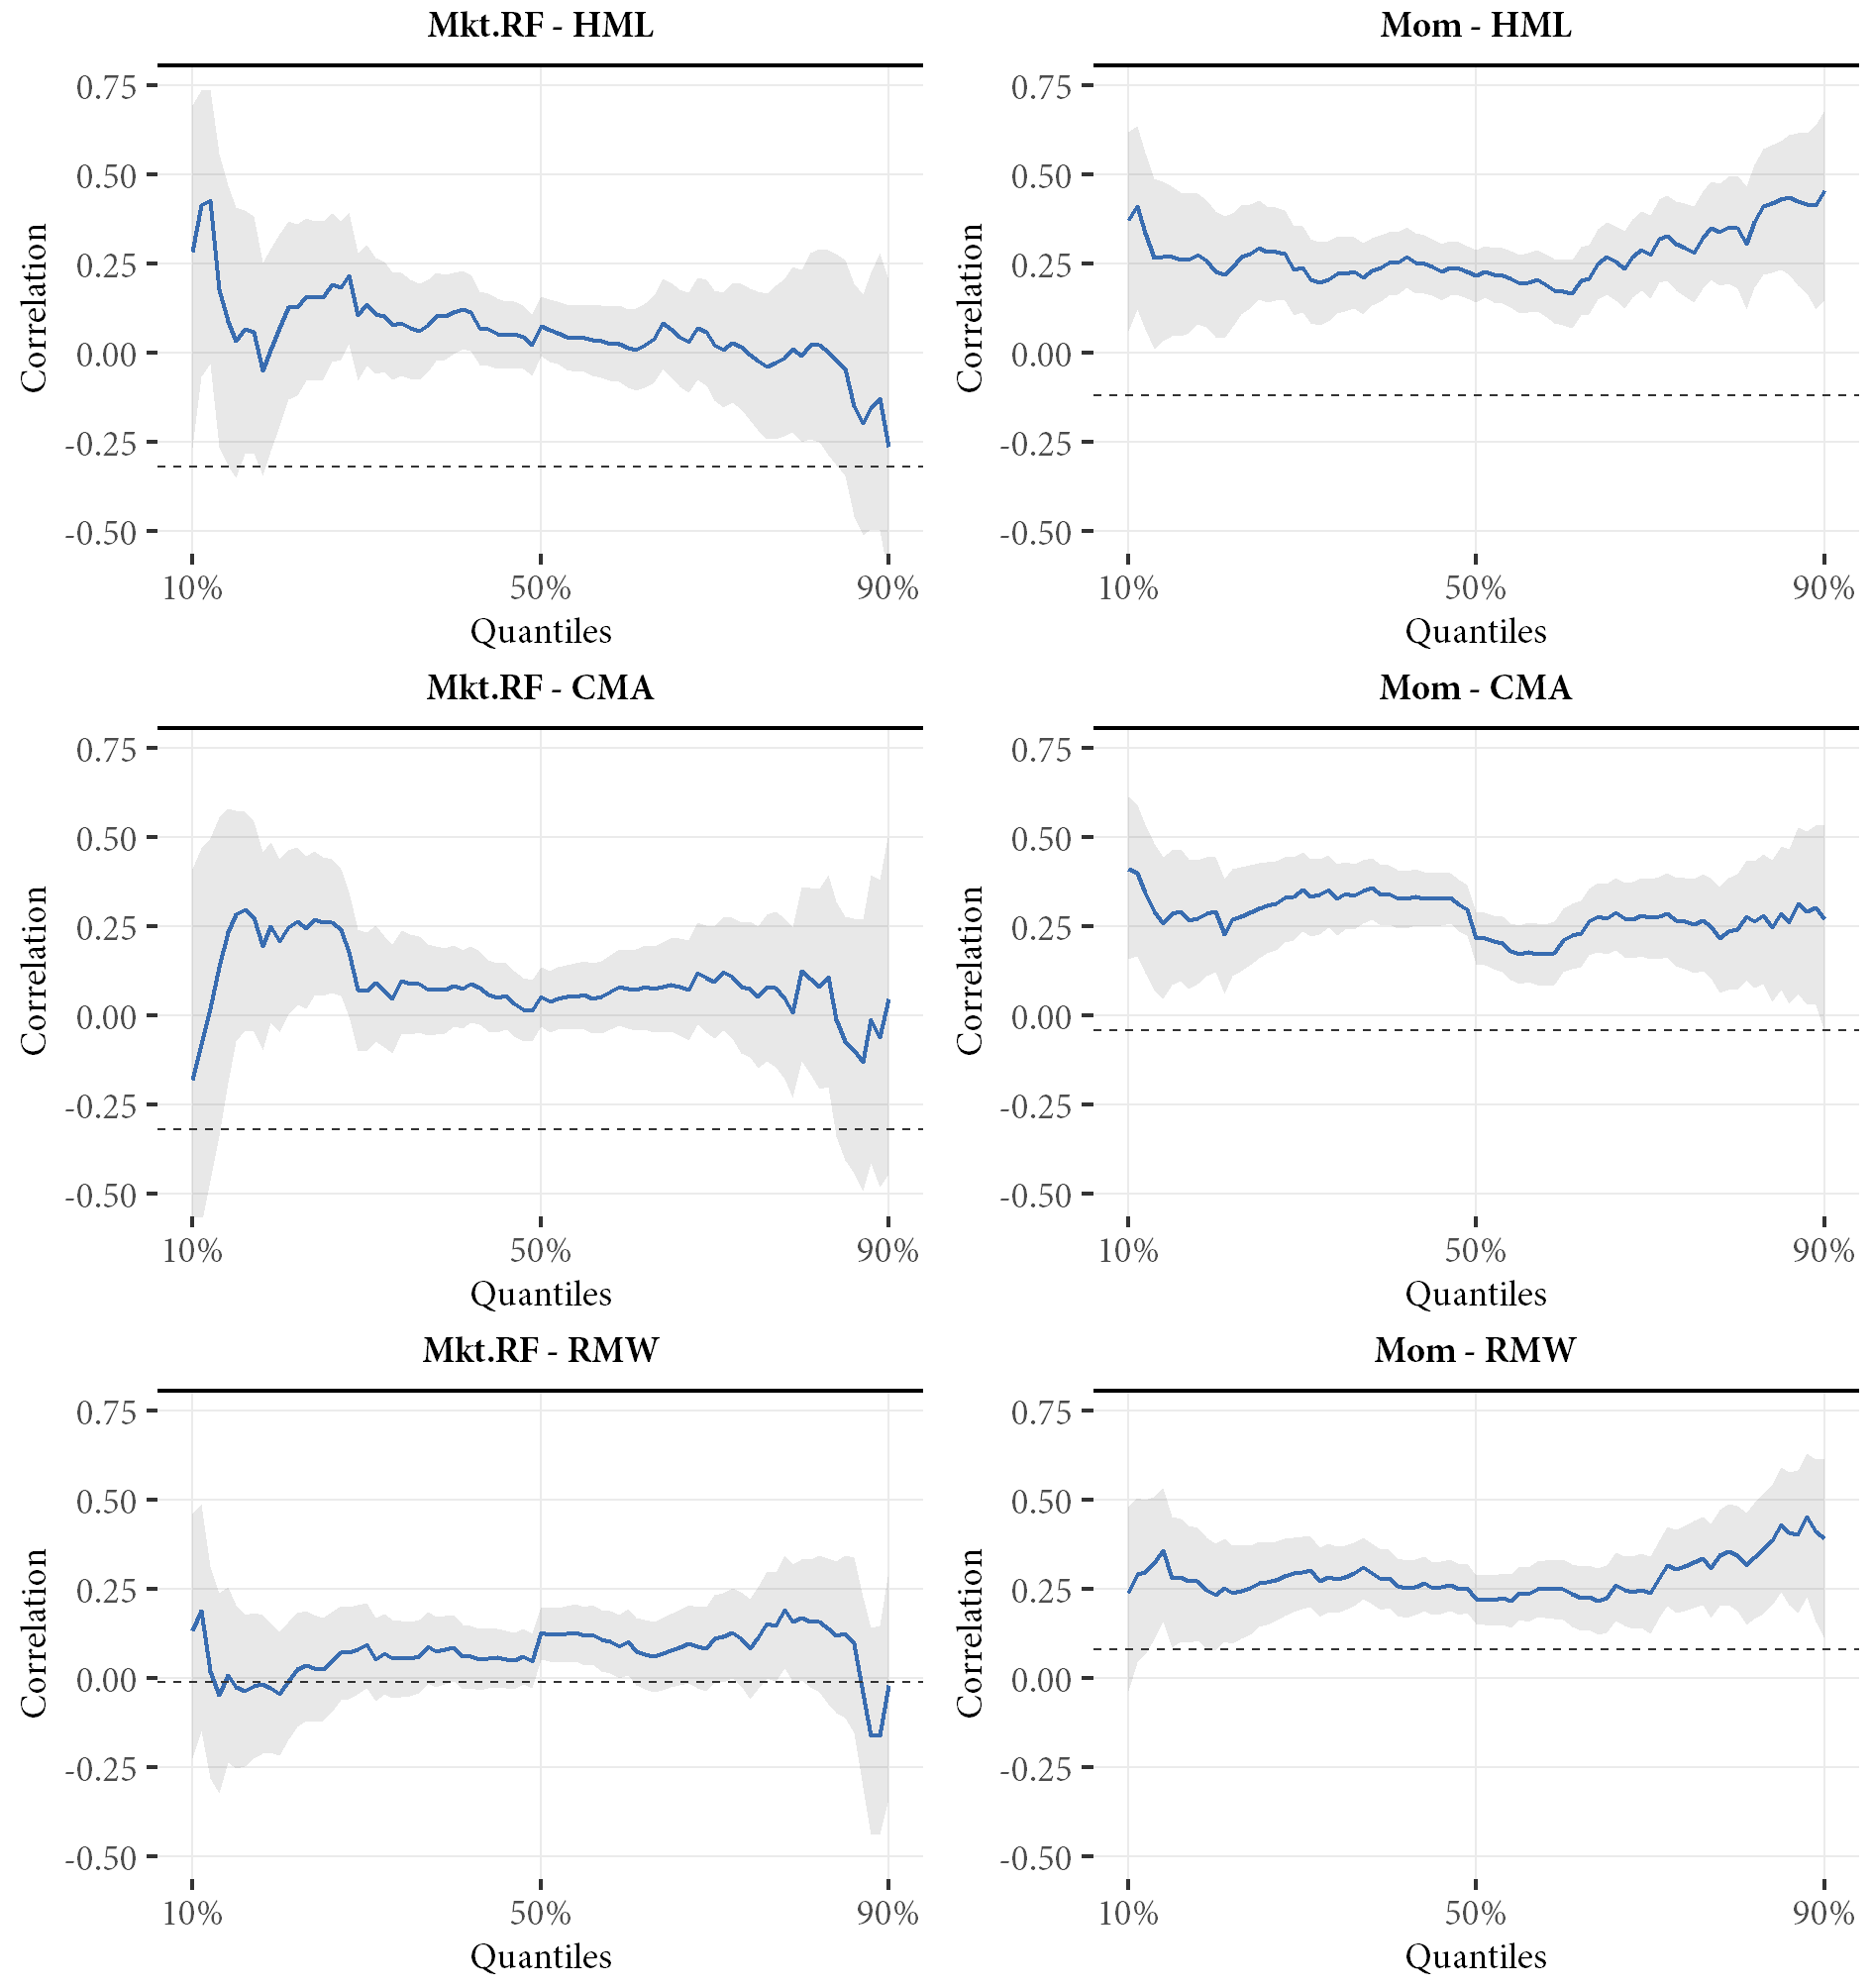
\includegraphics[scale=1]{graphics/threshold1.png}

  \caption{Threshold correlations of ARMA-GARCH standardized returns, fitted on full dataset (1963--2016). 95\% confidence bounds taking the model as given. The unconditional correlation is given by the dashed line.}
  \label{fig:threshold1}
\end{figure}

\begin{figure}[!ht]
  \ContinuedFloat
  \centering

  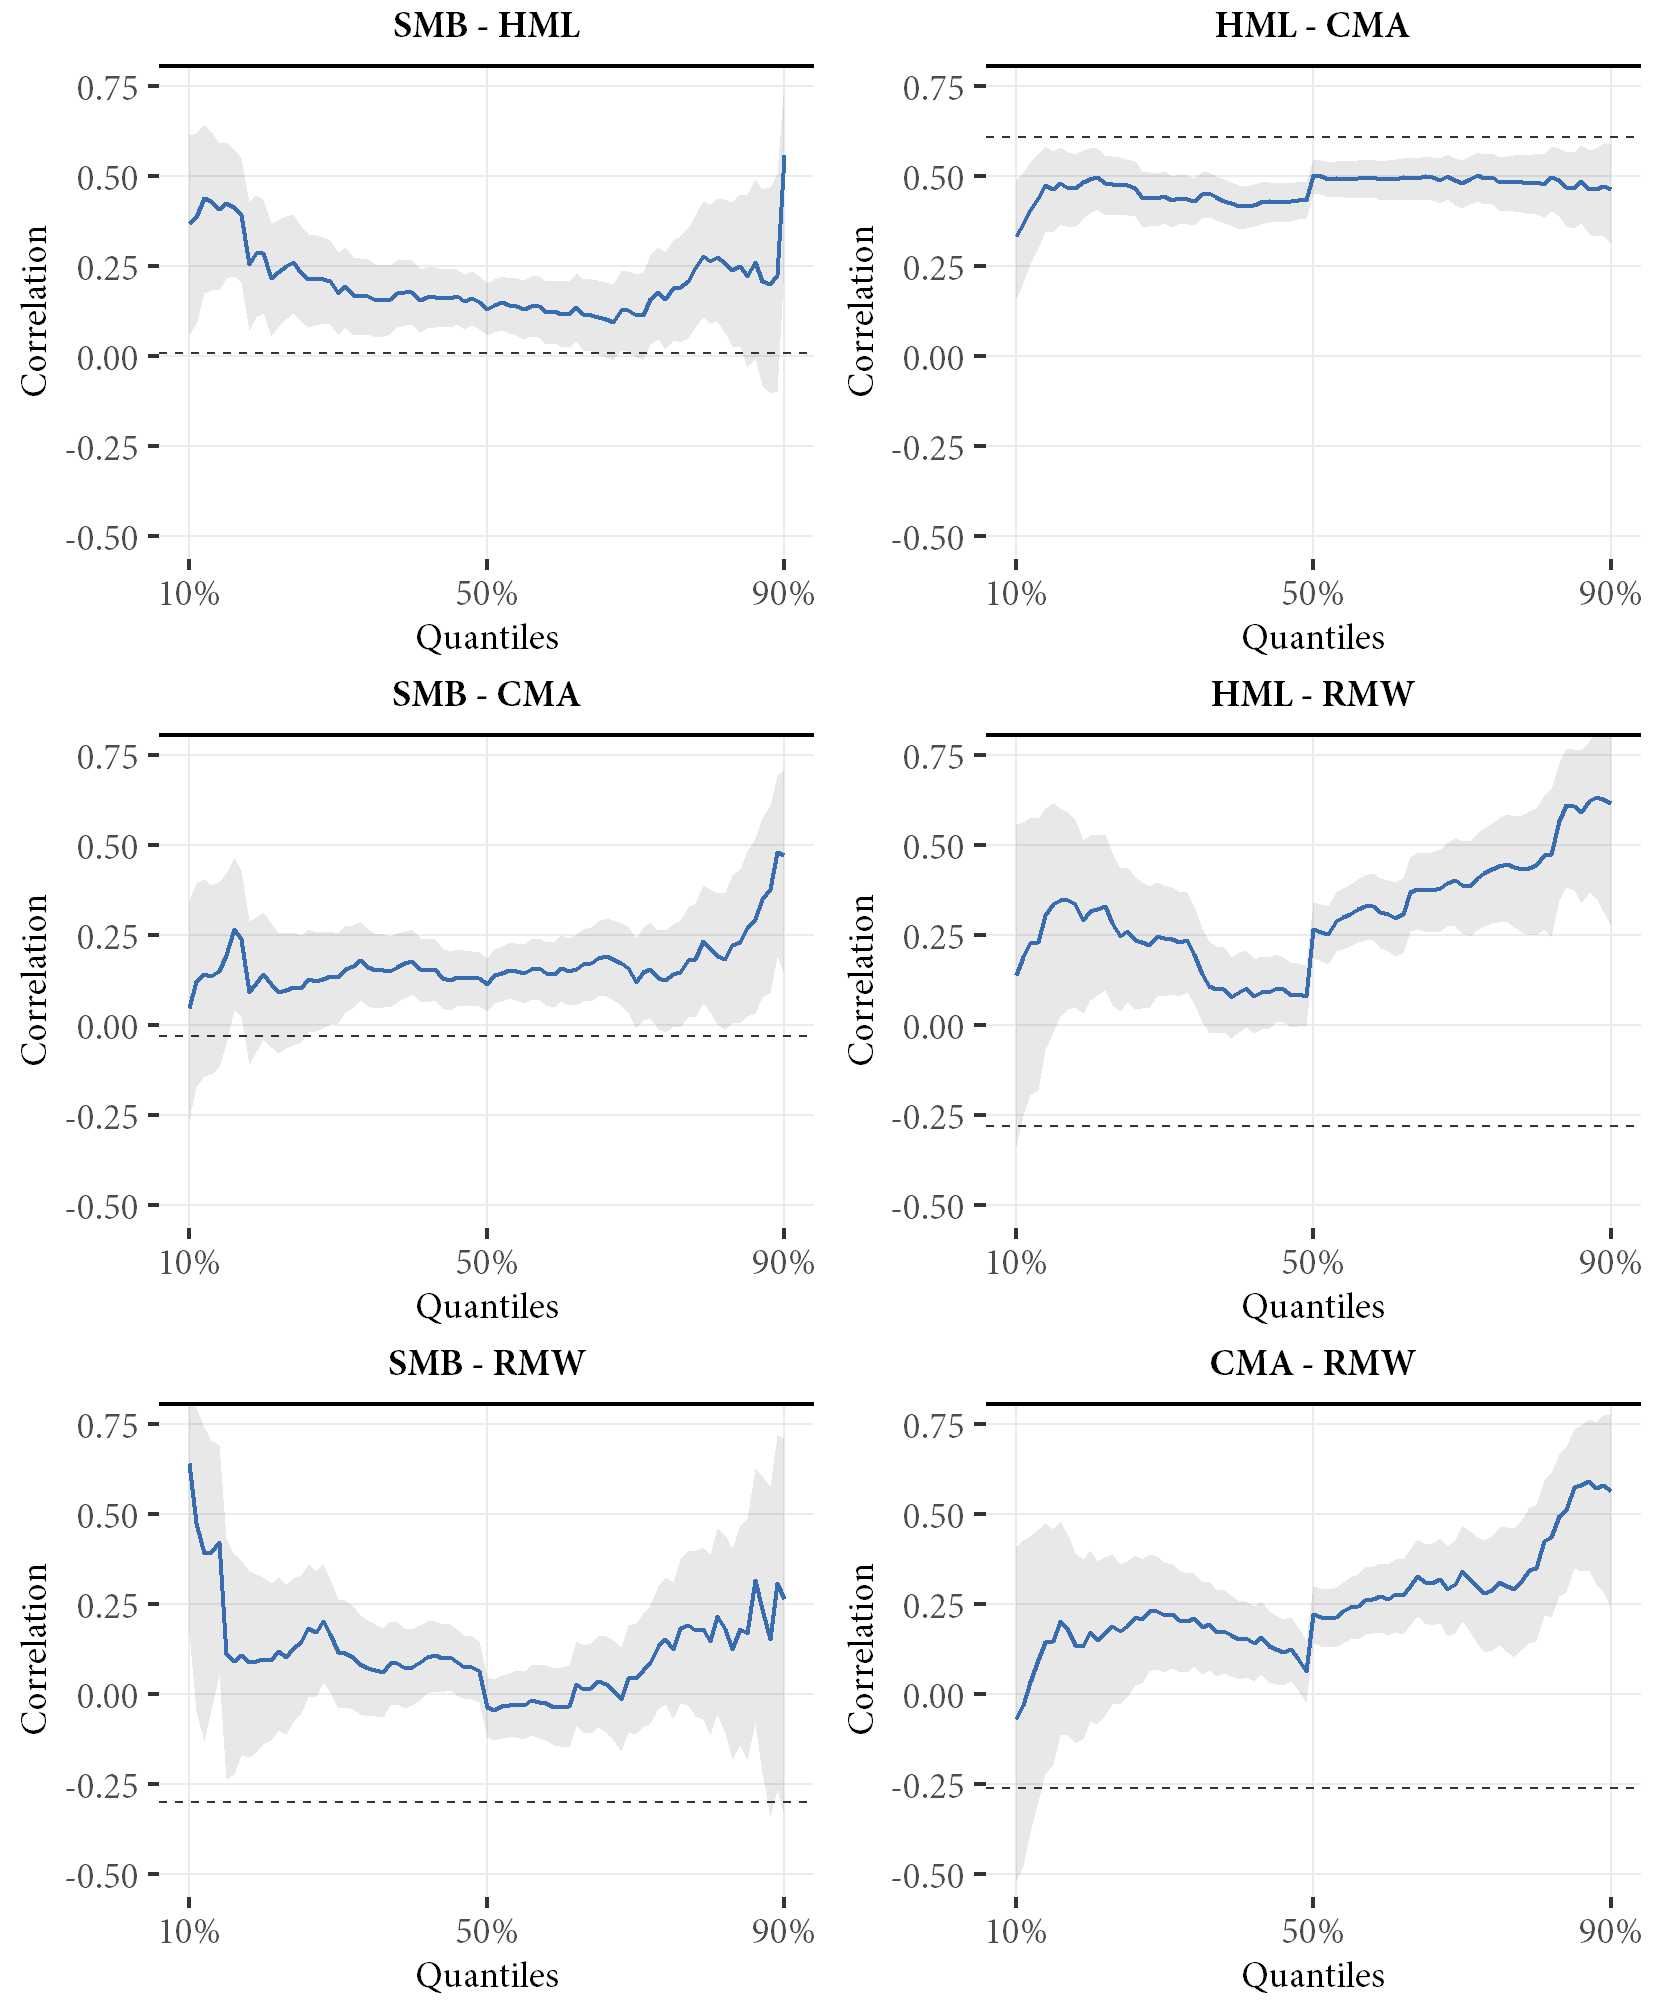
\includegraphics[scale=1]{graphics/threshold2.png}

  \caption{Threshold correlations of ARMA-GARCH standardized returns (cont.)}
\end{figure}

We now plot threshold correlations without the adjacent scatter graph. \autoref{fig:threshold1} displays threshold correlations for HML, CMA and RMW against eachother as well as against the the other factors Mkt-RF, SMB and Mom. We note that for most asset pairs, the threshold correlation is significantly different from the unconditional correlation coefficient, given by the dashed line.

We also note that there is asymmetry around the median for some factor pairs, including the Mom--CMA, RMW--HML, RMW--CMA, and to a lesser extent Mkt-RF--RMW asset pairs. For example, in the Mom-CMA asset pair, the threshold correlation jumps up for the first percentile below the median, indicating that the correlation is higher when both realize below the median than when both realize above the median. This type of asymmetric property, where downside (below the median) correlation is higher than upside correlation is unwanted, as it reflects a poorer diversification in bad times. 

Although estimated with substantial uncertainty, the threshold correlation do not seem to be constant as $p$ approaches either zero or one. For example, the Mkt-RF--HML asset pair seems to have a downward pattern, where correlation is the most positive in the lowest percentiles of residuals and the most negative in the highest percentile of residuals. In fact, this pattern is also unwanted from a diversification perspective, as series tend to coincide more in extreme negative events.

As do the original return series, all residual factor pairs exhibit unconditional correlation of near or below zero, except for the CMA--HML pair which exhibits a correlation in excess of $0.60$. Additionally, the threshold correlation estimate is much closer to this unconditional correlation -- suggesting that the tails of this pair is similar to the average.

While the patterns in threshold correlations are interesting, we are careful not to draw conclusions regarding diversification benefit based on solitary threshold correlation graphs -- our key point is that there seems to be tail dependence that should not be ignored in the copula specification. Tail dependence is only possible in the Student's \textit{t} copulae.

\subsubsection{Rolling Correlations}

We compute rolling 52-week correlations between the standardized returns of our ARMA-GARCH models according to the formula: 
\begin{align}
    RCorr(r_{i, t}, r_{j, t})_t^{52} = \frac{\sum^{t}_{t-51}(r_{i, t} - \bar{r}_i)(r_{j,t} - \bar{r}_j)}{\sqrt{\sum^{t}_{t-51} (r_{i,t} - \bar{r}_i)^2} \sqrt{\sum^{t}_{t-51} (r_{j,t} - \bar{r}_j)^2}}
\end{align}
where $r_i$, $r_j$ are the different pairs of the factor strategies' ARMA-GARCH residuals.\footnote{Rolling correlations for the returns themselves are available in the appendix.} Results are presented in ~\autoref{fig:rolling1}.
% plots
\begin{figure}[!ht]
  \centering
  \caption{Rolling correlations of ARMA-GARCH standardized returns \\ \quad \\
   Rolling correlations are fitted on the full dataset (1963--2016). 95\% confidence bounds taking the model as given. The unconditional correlation is given by the dashed line.}
  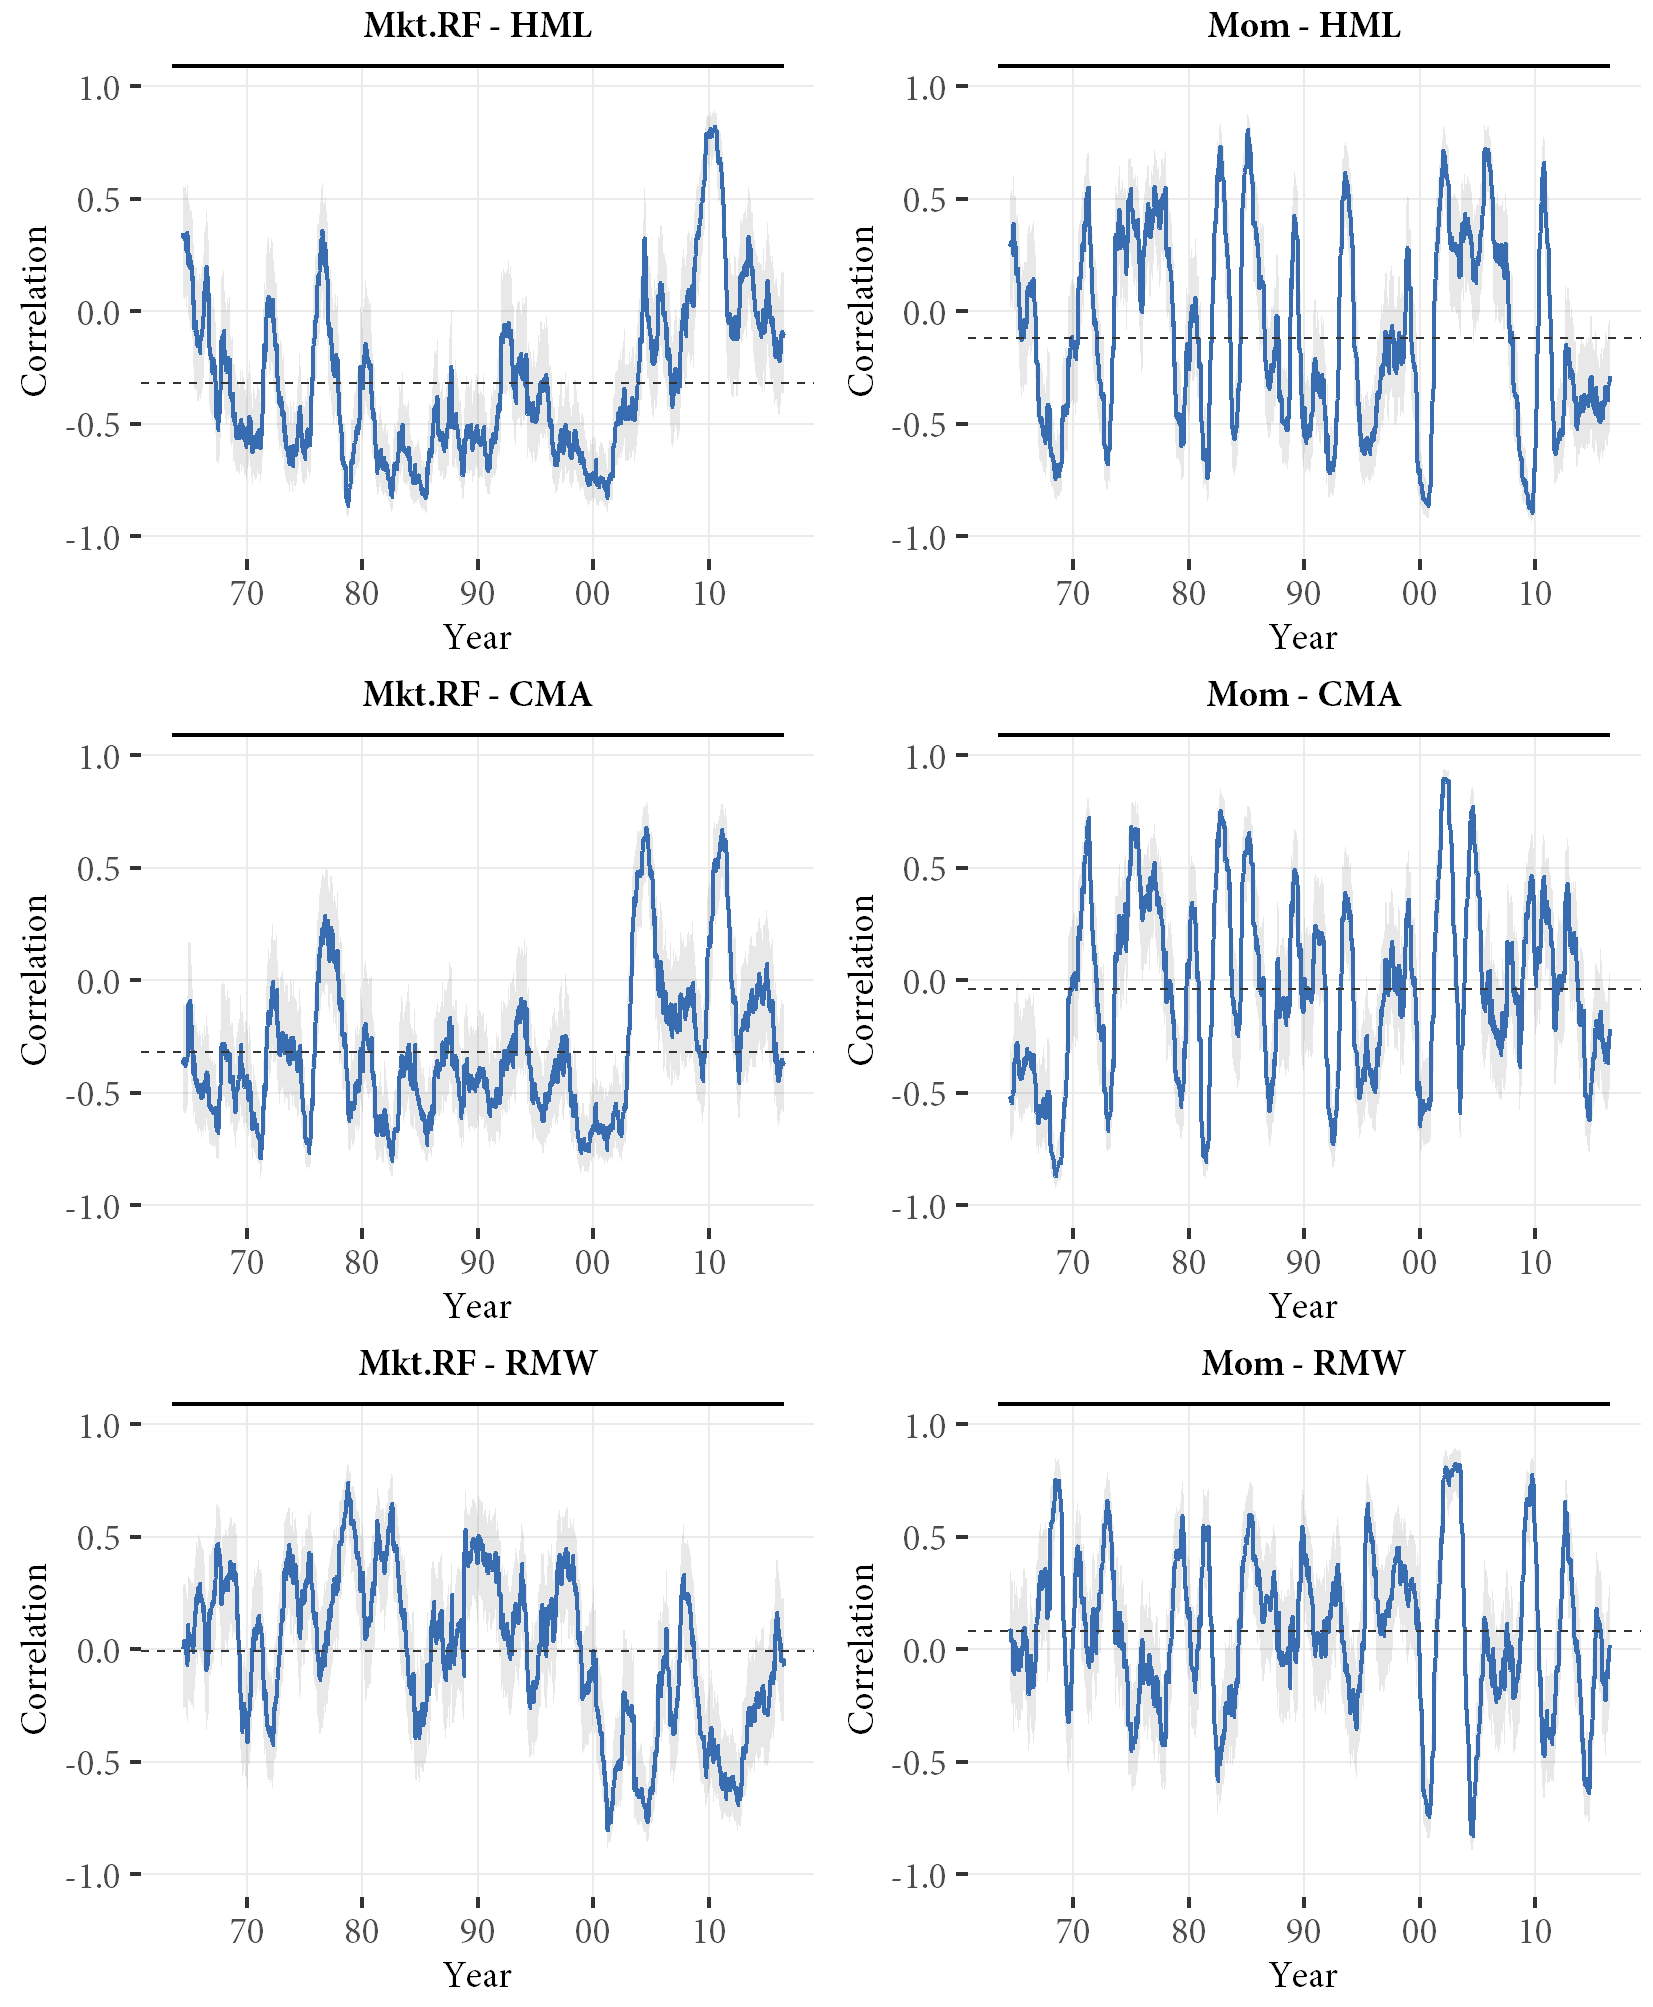
\includegraphics[scale=1]{graphics/rolling1.png}
  \label{fig:rolling1}
\end{figure}
\begin{figure}[!ht]
  \ContinuedFloat
  \centering
  \caption{Rolling correlations of ARMA-GARCH standardized returns (cont.)}
  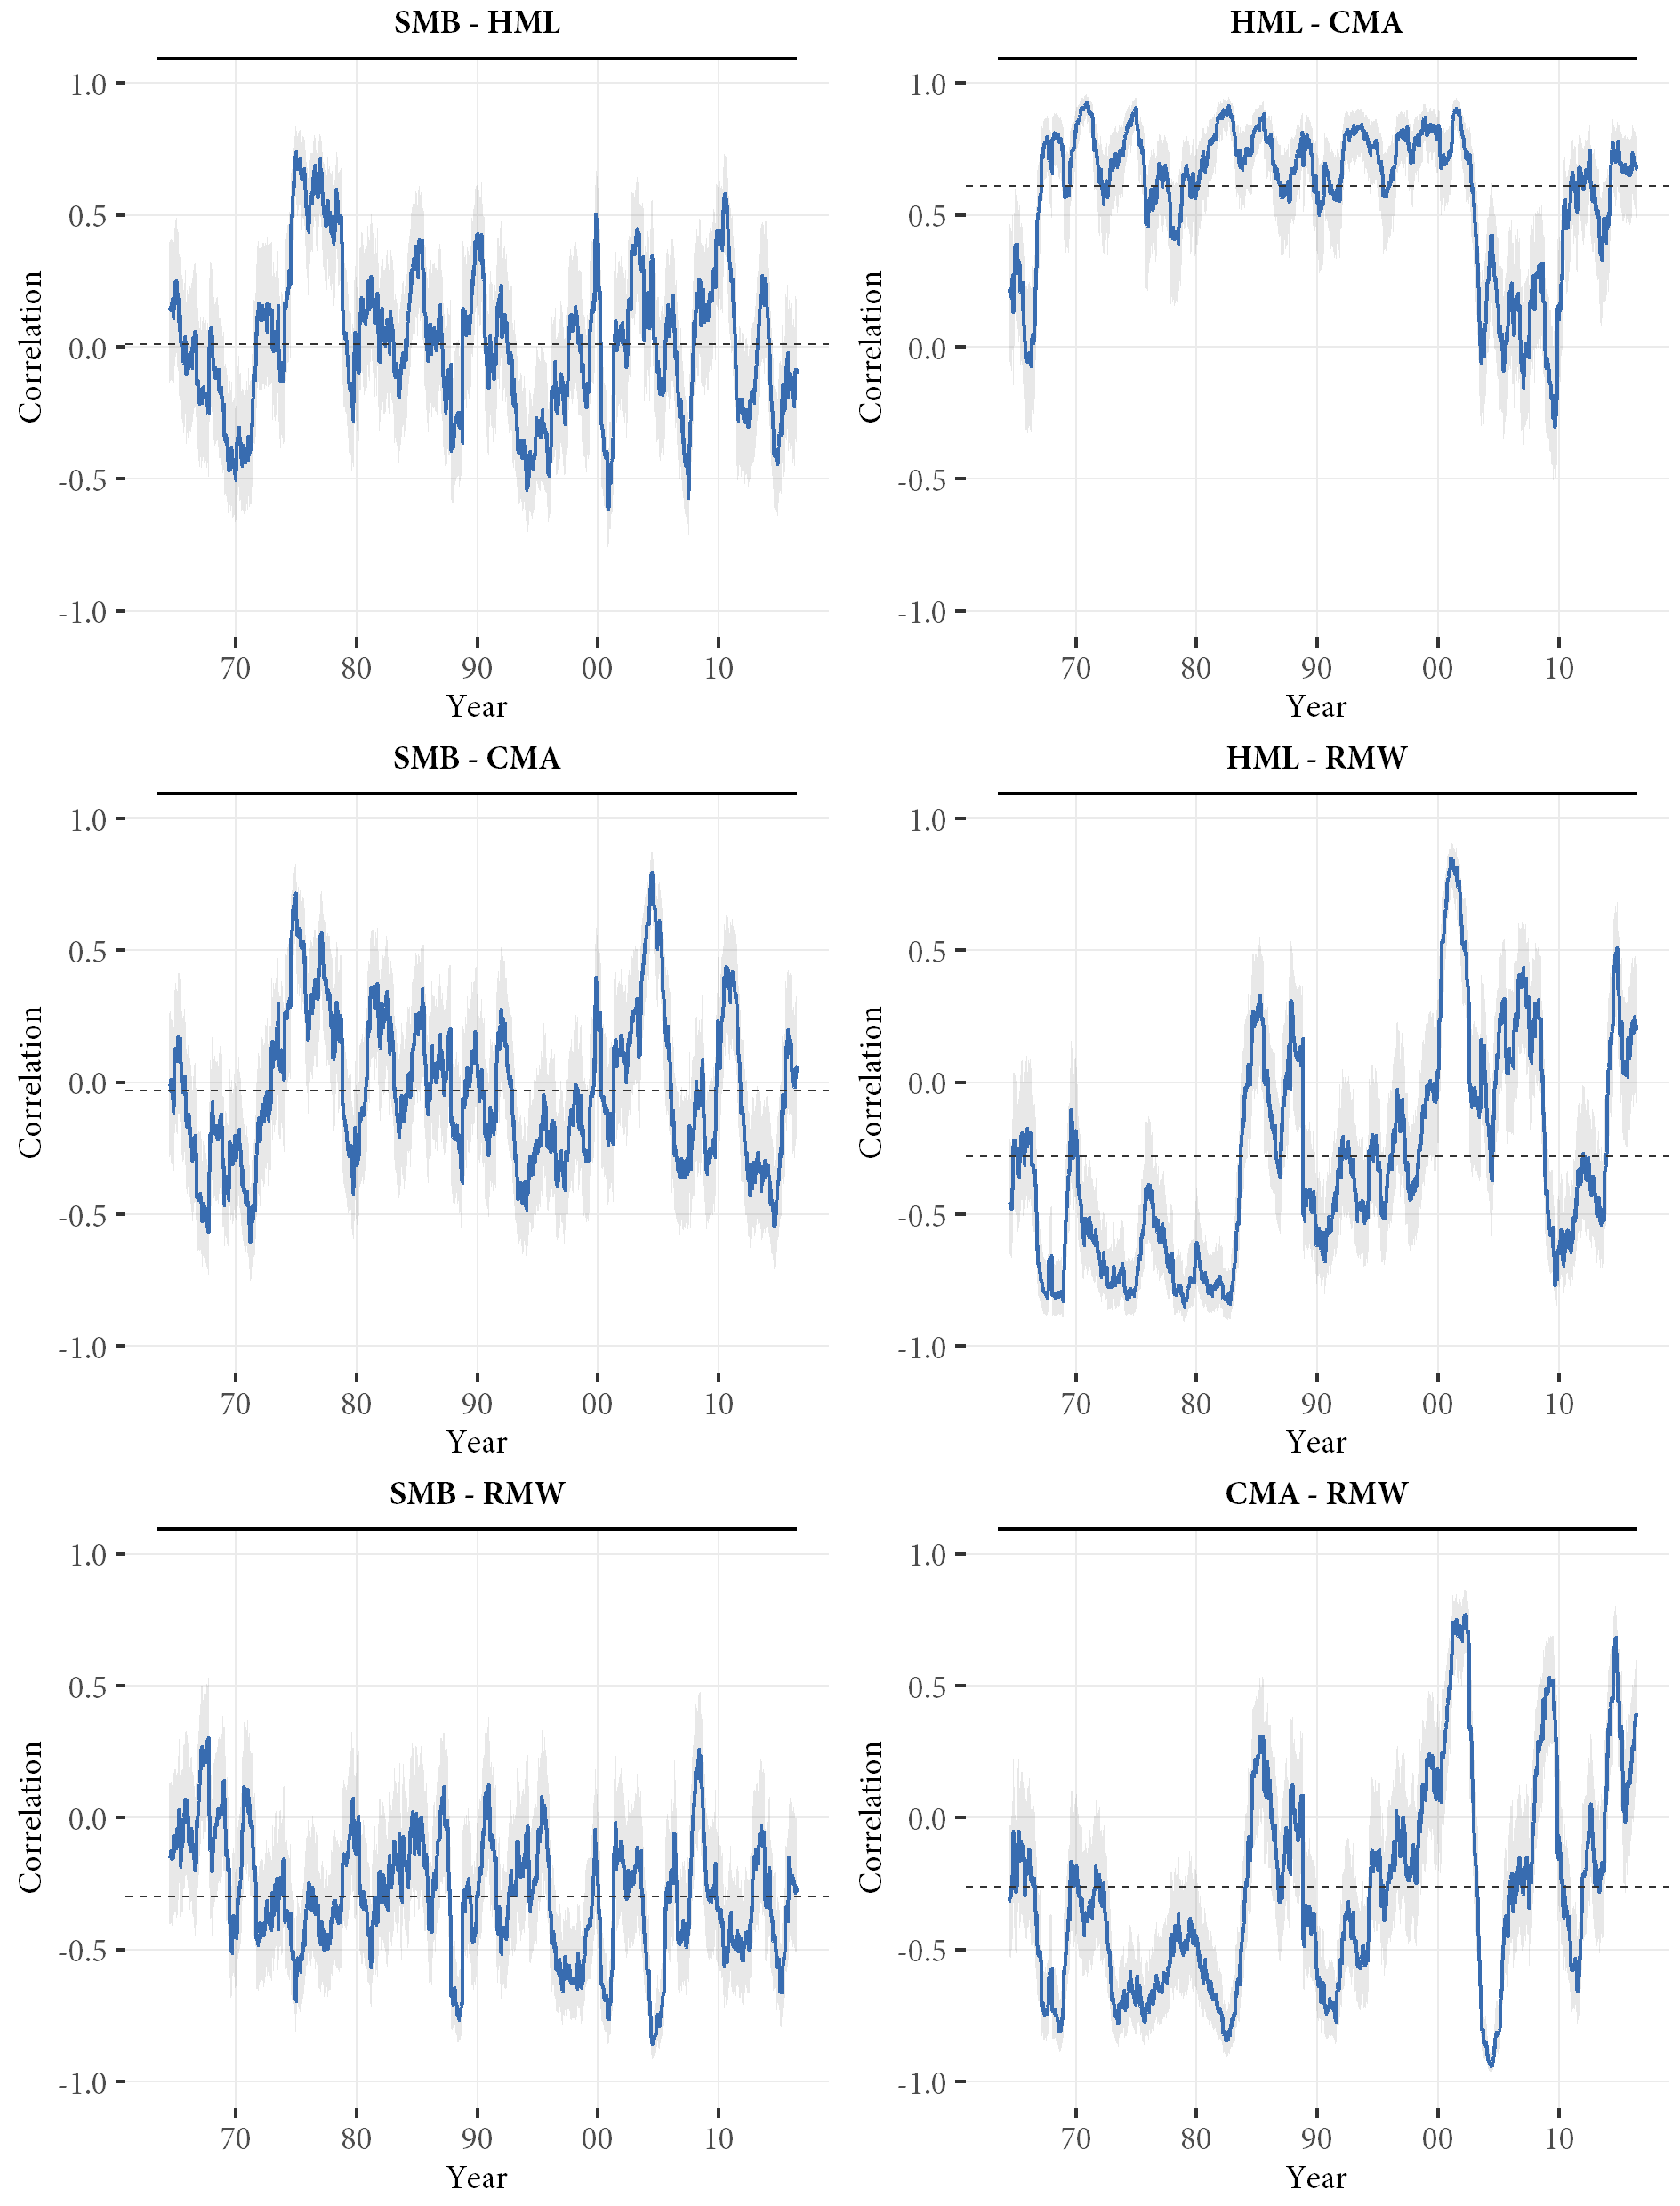
\includegraphics[scale=1]{graphics/rolling2.png}  
\end{figure}
% talk
First, we note that for most factor pairs, the rolling 52-week correlations are time-varying, and indeed appear to swing wildly. The unconditional correlation of Mkt--HML is negative in the studied time period, but rolling correlations range between -0.75 and 0.75. Also of note is the Momentum factor's rapid shifts between positive and negative correlations to the other factors. 

% Value and profitability in crisis times?
Second, by visual inspection, we see no obvious trend in the correlations between factor pairs, however, there are notable patterns around the 2000--2001 period -- the correlations of HML--RMW, CMA--RMW and Mkt--CMA appear to jump sharply. This is an indication that diversification benefits may be time-varying. Another interesting pattern is that the correlations of Mkt--RMW went down sharply around this period -- in line with the idea that profitable firms are stronger and better at weathering crises than the average firm~\autocite{NovyMarx2013}. The 2000--2001 period may represent a structural break in the dependency patterns between factors, with the appearance of persistent differences before and after -- however, there is not enough post-2000 data to support such a conclusion, yet.

Third, the HML and CMA factors again stand out as different to other factor pairs. The unconditional correlation is much closer to the rolling estimates than for other factor pairs, with a dip in the 2000--2010 period that appears to have gone away. Clearly, the HML--CMA pair is the most strongly correlated factor pair, even when considering specific time periods in the data.

Our key takeaway from the rolling correlations is that there seems to be persistency in the time-variation in correlations. This could be incorporated in the copula specification, which then needs to have a time-varying correlation matrix $\Psi_t$.

% \subsubsection{Takeaways from Analysis of Multivariate Dependence}

% Univariate residuals appear to be white noise series with no remaining autocorrelation or volatility clustering. However, there is important dependence between residuals of different strategies. First, threshold correlations show that there is tail dependence -- in times when factor pairs simultaneously realize in their best and worst percentiles, correlations are significantly different from the unconditional correlations. In fact, threshold correlations are substantially higher than the unconditional correlations, which indicates that diversification benefits are smaller than expected when factors simultaneously experience bad (or good) times. Second, rolling correlations show that correlations between series are highly time-varying and seem to exhibit persistence. A copula model that incorporates both tail dependence and time-varying dependence is likely to improve on the description of joint returns.

% Both analyses also show that the HML-CMA asset pair is quite different from the other pairs, exhibiting a much higher and more stable dependence. Differently put, they look quite similar as opposed to any other factor pair, and the merit of including both in factor portfolios seems more unclear.

\label{sub:threshold_and_rolling_correlations_of_residuals}

% subsection threshold_and_rolling_correlations_of_residuals (end)

%!TEX root = ../main.tex
\subsection{Copula specification and estimation results}
Given the results of the dependence structure of residuals, we now discuss the best choice of copula model and present estimation results of the six competing copula specifications.

\subsubsection{Interpreting and choosing copula specification}

The interpretation of the copula parameterization is closely associated to the structure of multivariate dependence. By different restrictions on the parameters in the DAC model, we are able to activate or deactivate certain features of the copula: First, the degree of freedom parameter $nu_c$ is to be interpreted as a the measure of tail dependency. When $nu \neq 0$, the lower and upper tails of the joint distribution are fatter than in the normal case, which is coherent with the evidence from threshold correlations. Second, the skewness parameters $\gamma_{c,i}$ are to be interpreted as the extent of asymmetry in the correlation structure. When $\gamma \neq 0$, there is asymmetry in correlations, which is also coherent with the earlier threshold correlation analysis. Third, the $\alpha$ and $\beta$ parameters determine whether the copula generates time-varying correlations. If $\alpha \neq 0$ and $\beta \neq 0$, the copula is dynamic, which is consistent with the findings of the rolling correlation analysis. An overview of the six copula models is given in \autoref{fig:conceptual}.

%!TEX root=../../main.tex

\begin{table}
  \centering
  \footnotesize
  \renewcommand{\arraystretch}{1.2}

  \caption{Conceptual matrix of copula parameterizations}

  \begin{tabularx}{0.80\textwidth}{@{} lc c >{\centering}Xc >{\centering}Xc >{\centering\arraybackslash}X}
    \toprule
      & && \textbf{Normal} && \textbf{Symmetric \emph{t}} && \textbf{Skewed \emph{t}} \\
      \cmidrule{4-4}
      \cmidrule{6-6}
      \cmidrule{8-8}
      & && $\nu_c = \infty$   && $\nu_c < \infty$   && $\nu_c < \infty$ \\
      & && $\gamma_{i,c} = 0$ && $\gamma_{i,c} = 0$ && $\gamma_{i,c} \neq 0$ \\
      \cmidrule{4-8}
    \cmidrule{1-2}
    \multirow{2}{*}{\textbf{Constant}} & $\alpha = 0$ && Constant && Constant && Constant \\
                              & $\beta = 0$  && Normal   && Symmetric \emph{t} && Skewed \emph{t}      \\
    \cmidrule{1-2}
    \multirow{2}{*}{\textbf{Dynamic}}  & $\alpha > 0$ && Dynamic  && Dynamic && Dynamic \\
                              & $\beta > 0$  && Normal   && Symmetric \emph{t} && Skewed \emph{t}      \\
    \bottomrule
  \end{tabularx}
% ()
%   \begin{tabularx}{\textwidth}{@{\extracolsep{5pt}} c c c c X c X c @{}}
%     \toprule
%   				&			& &	\textbf{Normal}	&	&	\textbf{Student's \textit{t}}	&	&	\textbf{Asymmetric Student's \textit{t}} \\
%   				\\
%   				&			& & 	$\nu = \infty$	&	&	$\nu > 0$	& 	&	$\nu > 0$ \\
%   				&			& & 	$\gamma = 0$	&	&	$\gamma = 0$	& 	&	$\gamma \neq 0$ \\
%           \\
%     \cmidrule{4-8}
%     \\
%      \textbf{Constant} &  & & \text{Constant normal copula} & & \text{Constant symmetric \textit{t} copula} & & \text{Constant asymmetric \textit{t} copula} \\
%      \\
%     	&	$\alpha = 0$  &		&	\textit{Constant correlations but} & & \textit{Constant correlations and} & & \textit{Constant correlations and} \\
%        & $\beta = 0$ & & \textit{no tail dependence} & & \textit{symmetric tail dependence} & & \textit{asymmetric tail dependence} \\
%     \\
%     \cmidrule{4-8}
%     \\
%      \textbf{Dynamic} &  & & \text{Dynamic normal copula} & & \text{Dynamic symmetric \textit{t} copula} & & \text{Dynamic asymmetric \textit{t} copula} \\
%      \\
%       & $\alpha > 0$  &   & \textit{Dynamic correlations but} & & \textit{Dynamic correlations and} & & \textit{Dynamic correlations and} \\
%        & $\beta > 0$ & & \textit{no tail dependence} & & \textit{symmetric tail dependence} & & \textit{asymmetric tail dependence} \\
%     \\
%     \bottomrule
%   \end{tabularx}

  \label{tab:conceptual}	
\end{table}


\subsubsection{Copula estimation results}

We estimate constant and dynamic normal, symmetric and asymmetric copula models on the full dataset of GARCH uniform residuals. Results are presented in~\autoref{tab:copula_estimation}. First, we examine the choice between a normal, symmetric \textit{t} or asymmetric \textit{t} copula. We note that $\nu_c$ is clearly significant and suggests a Student's \textit{t} model with tail dependence over the normal model. Second, we examine the asymmetric specification and find that few of the $\gamma_c$ estimates appear significant, indicating that the asymmetry is hard to capture or not consistent enough to merit modeling. This is supported by the relatively small improvement in log-likelihood by going from a symmetric to asymmetric copula and the fact that the BIC criterion prefers the symmetric model in the dynamic case. 

Second, we examine the choice between a constant and dynamic copula correlation matrix. There is a significant improvement in log-likelihood and BIC when moving from a constant to a dynamic copula, which suggests that time-varying dependence shown by rolling correlation is captured, which improves the model's fit. We also find a high persistence of the correlation process, as $\alpha + \beta$, is close to a unit root.

In summary, we find that the dynamic symmetric Student's \textit{t} copula is the best specification, as it has the lowest BIC, well defined parameters, and is strongly supported by the dependence pattern showcased by threshold and rolling correlation analyses. While the asymmetric Student's \textit{t} is an interesting model, we believe that the asymmetry patterns in data are too irregular to capture well in a copula model with only one asymmetry parameter for each series (this is further discussed in the subsequent robustness discussion, see \autoref{sub:05_robust}).
%what model do we retain (and why)

% section modeling_of_factor_returns (end)
